\documentclass{article}
\DeclareMathSizes{10}{10}{7}{7}
\usepackage{amsmath}
\usepackage{ amssymb }
\usepackage{tikz, graphicx}
\usepackage{geometry}
\usepackage[makeroom]{cancel}
\usepackage[export]{adjustbox}
\DeclareMathOperator{\sech}{sech}
\usepackage{subfig}
\usepackage{hyperref}
\hypersetup{
    colorlinks=true,
    linkcolor=blue,
    filecolor=magenta,      
    urlcolor=blue,
    }
\usepackage{float}
\restylefloat{table}

\geometry{legalpaper, margin=0.7in}

\title{Noize net}
\author{Liam Watson}
\begin{document}
\maketitle

\section{Intorduction to Neural networks}
\label{sec:intro}
Before we procede to the more advanced recurant neural network let us begin with an abbrevated coveradge of neaural networks and the convepts underpining them. 
\subsection{Perceptrons}
\label{sec:peceptrons}
The simplest unit of a neural network is, as the name suggests a neuron or more commonly a peceptron. In it's simplest form a peceptron recieves an input, performs some calculation and produces output.
\begin{figure}[h]
\caption{Peceptron showing N input variables, N weights and a bias}
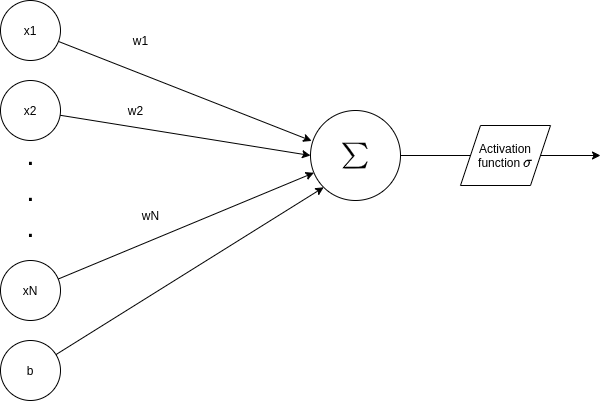
\includegraphics[scale=0.5]{peceptron.png}
\end{figure}
Given these inputs and bias we can adjust weights and bais to satisfy our desired output after summation and activation function (\ref{sec:activationfuncs}). 

\subsection{Multi layer peceptrons}
\label{sec:mlp}
Peceptrons, however, are not powerful in this form, rather we only begin to see the utility when we start connecting them together in a mesh much like neurons in the brain. In figure two we can see a depiction of this with weights represented as line thickness (\autoref{fig:mlp}).
\begin{figure}[h]
\caption{Image of a simple neural network archutecture with 8 inputs two hidden layers and four output neurons}
\label{fig:mlp}
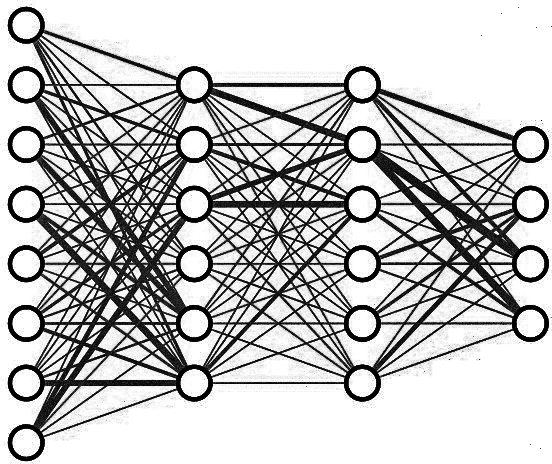
\includegraphics[scale=2]{nn.jpg}
\href{https://www.youtube.com/watch?v=aircAruvnKk&ab_channel=3Blue1Brown}{Sorce}
\end{figure}
\subsection{Gradient decent}
Now we need a way to determine the peceptron weights, for this we use Gradient decent. There are many adaptions of gardient descent that aim to optimize its computational performance or over come some issue with converging to a poory optimised solution such as Fast gradient methods or momentum adapted gradient descent. \\
The aim of gradient descent is to itteratively optimize the peceptron weights to converge on a local minimum by taking steps in the direction of steepest descent, after many itterations we will find that the networks weights are well optimised for some goal. However we may find that a local minimum is not sufficient for our purposes and as such may need to employ some hyperparameter tuning such as changing the the step size we take or adding momentum in the hopes that we converge to a more optimal solution.
\label{sec:gradientDecent}
\begin{figure}
\caption{A plot of $f(x,y) = \sin(x) + \sin(y)$ with a path showing gradient decent steps}
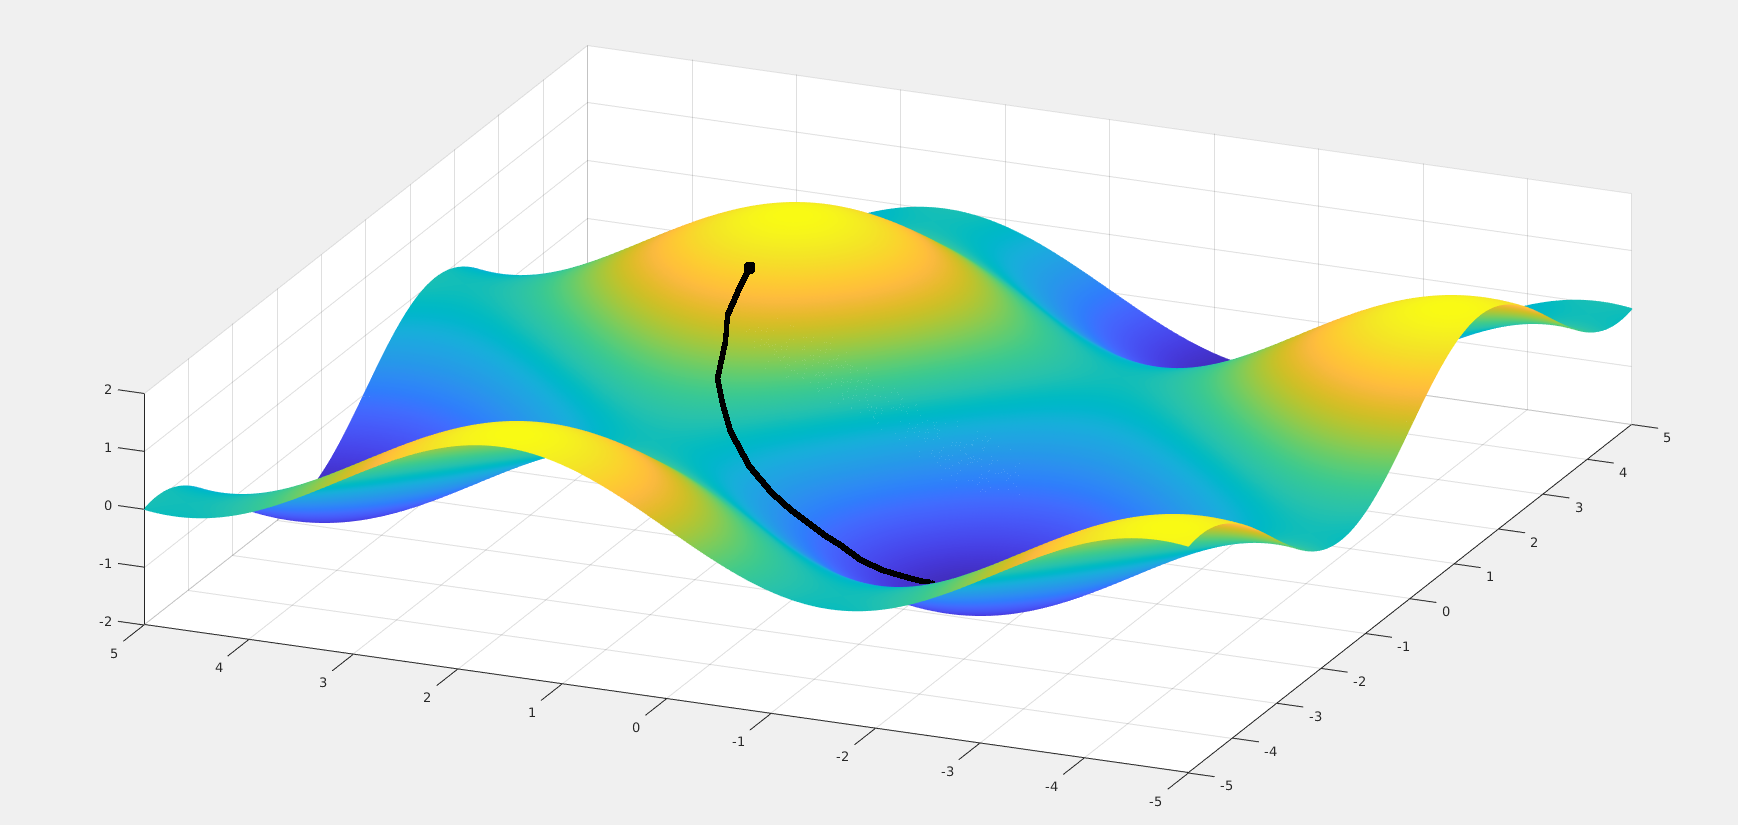
\includegraphics[scale=0.3]{mesh.png}
\end{figure}
\subsection{Activation functions}
Now we will discuss, much like with a biological neuron, how will a neuron decide to acivate or not. There are many functions that are used in the literature but here we give give a quick overview of the most common functions and their uses. The purpose of an activation function is to format the output of a peceptron, we begin with the most elementary of these functions (excluding the identity function defined as $f(x) = x$. 
\begin{enumerate}
\item The binary step function 
Definition:
\begin{align*}
f(x) = 
\begin{cases}
 1 & \text{if } x > 0 \\
 0 & \text{if } x \leq 0 \\
\end{cases}
\end{align*}
The binary step function is primarly used for true, falue classification where the result is not a probability but a certanty. Beyond this this activation function has limited use in modern neural networks, hoever it should be noted that it is very computationally efficient. 
\item Rectified Linear Unit(ReLU)
Definition: 
\begin{align*}
f(x) =
\begin{cases}
 0 & \text{if } x \leq 0 \\
 x & \text{if } x > 0 \\
\end{cases}
\end{align*}
The ReLU Function finds much use dispite its simplicity mostly due to its computational efficiency when compared to the more complex activation functions. ReLU reduces the input domain to only non-negative numbers which can be useful in cases where one wishes to disregard such values. 
\item Sigmoid
Definition: 
\begin{align*}
f(x) =
\begin{cases}
 0 & \text{if } x \leq 0 \\
 x & \text{if } x > 0 \\
\end{cases}
\end{align*}
\item Softmax
Definition: CHANGE THIS
\begin{align*}
f(x) =
\begin{cases}
 0 & \text{if } x \leq 0 \\
 x & \text{if } x > 0 \\
\end{cases}
\end{align*}

\end{enumerate}

\label{sec:activationfuncs}

\subsection{Error functions}
\label{sec:error}

\subsection{Feed forward}
\label{sec:forward}

\subsection{Back propication}
\label{sec:back}


\section{Intorduction to Recurrant Neural Networks}
\label{sec:intoRNNs}
\subsection{RNN concepts}
\label{sec:RNNS}
\subsection{LSTM}
\label{sec:LSTM}

\section{Noize net}
\label{sec:nn}
\subsection{Data and preprocessing}
\label{sec:data}
\subsection{Architecture}
\label{sec:arch}
\subsection{Implimentation}
\label{sec:impl}
\subsection{Results}
\label{sec:results}
\subsection{Conclusion}
\label{sec:conclusion}

\section{References}

\end{document}